\documentclass[border=10pt]{standalone} 
\usepackage{verbatim}
\begin{comment}
\end{comment}
\usepackage{tikz}
\tikzset{
  treenode/.style = {shape=rectangle, %rounded corners,
                     draw, align=center,
                     top color=blue!5, 
                     bottom color=blue!5},
  root/.style     = {treenode, 
  						font=\large, 
                        top color=white!5, 
                        bottom color=white!30},
  env/.style      = {treenode, font=\ttfamily\normalsize},
  red/.style      = {treenode, font=\ttfamily\normalsize, 
  					top color=red!5, 
  					bottom color=red!5},
  green/.style      = {treenode, font=\ttfamily\normalsize, 
  					top color=green!5, 
  					bottom color=green!5},
  dummy/.style    = {circle,draw}
}
\begin{document}
\tikzstyle{level 1}=[level distance=1.5cm, sibling distance=2.5cm]
\tikzstyle{level 2}=[level distance=2.5cm, sibling distance=6cm]
\tikzstyle{level 3}=[level distance=2.5cm, sibling distance=3.5cm]
\tikzstyle{level 4}=[level distance=2.5cm, sibling distance=1.8cm]
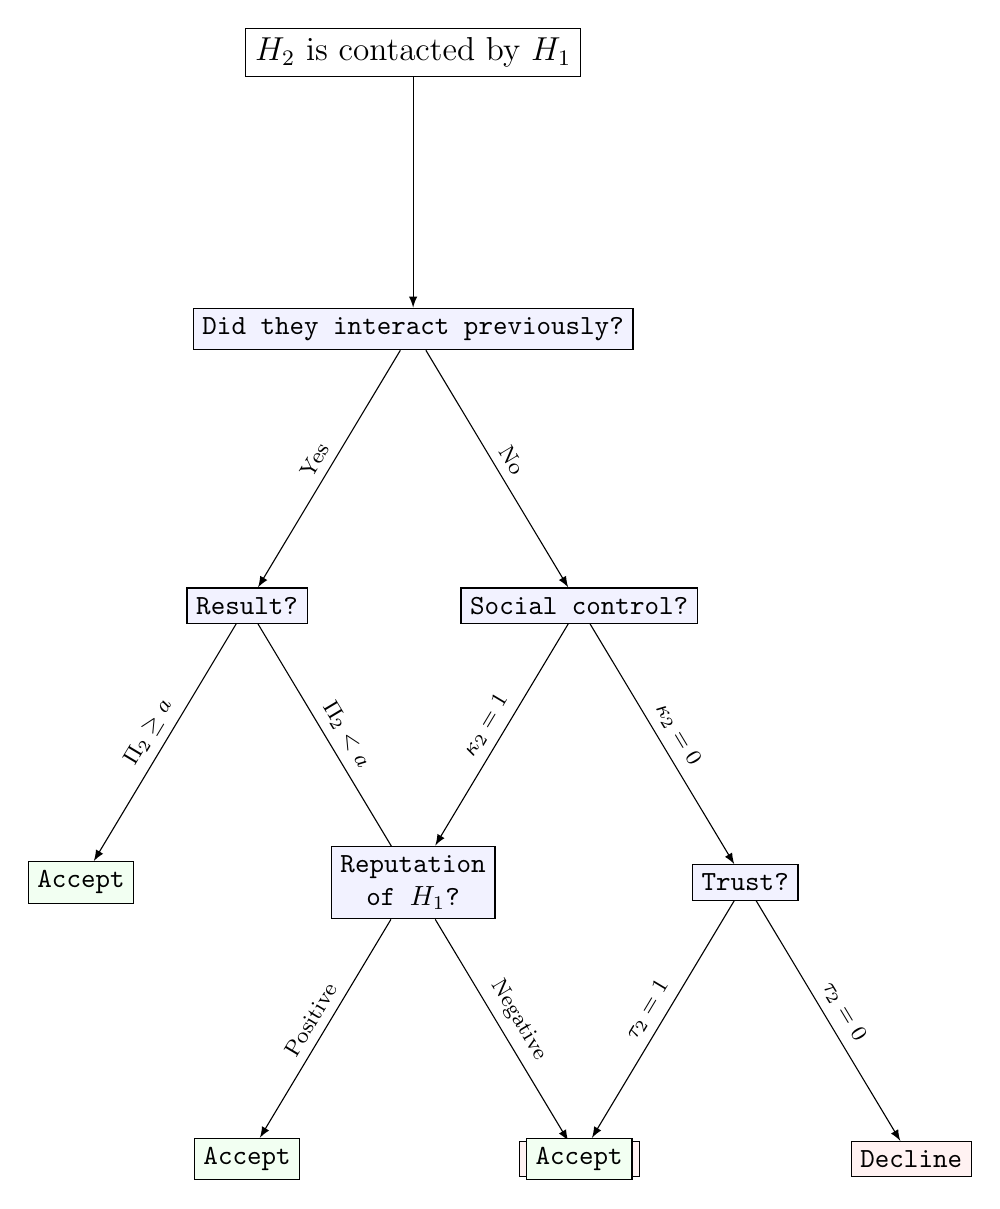
\begin{tikzpicture}
  [
    grow                    = down,
    sibling distance        = 12em,
    level distance          = 10em,
    edge from parent/.style = {draw, -latex},
    every node/.style       = {font=\footnotesize},
    sloped
  ]
  \node [root] {$H_2$ is contacted by $H_1$}
    child { node [env] {Did they interact previously?}
      child { 
      node [env] {Result?}
      	child { node [green] {Accept} 
      	edge from parent node [above] { $\Pi_2\geq a$ } }
      	child { node [red] {Decline}
      	edge from parent node [above] { $\Pi_2< a$ } }
      edge from parent node [above] { Yes } }  
      child { 
      node [env] {Social control?}
      	child { node [env] {Reputation\\ of $H_1$?} 
      		child { 
            	node [green] {Accept}
      			edge from parent node [above] { Positive } 
                }
      		child { 
            	node [red] {Decline}
      			edge from parent node [above] { Negative } 
                }
      	edge from parent node [above] { $\kappa_2=1$ } 
        	} 
      child { node [env] {Trust?}
      child { node [green] {Accept}
      edge from parent node [above] { $\tau_2=1$ } }
      child { node [red] {Decline}
      edge from parent node [above] { $\tau_2=0$ } }
      edge from parent node [above] { $\kappa_2=0$ } }
        edge from parent node [above] { No } }
        };
\end{tikzpicture}

\end{document}